\section{Observer-Muster}
\subsection{Problemstellung}
\begin{itemize}
	\item Wetterstation liefert Daten (Luftdruck, Temperatur, etc.).
	\item Gefragt ist ein WetterDaten-Objekt. 
	\item Diverse Anzeigeger"ate sollen in der Lage sein, sich die Daten vom WetterDaten-Objekt zu ziehen 
und entsprechend darzustellen. Problematisch wird es, wenn verschiedene Anzeigeger"ate nur 
bestimmte Daten anzeigen sollen. 
	\item Besonderes Augenmerk bei dieser Aufgabe, die Daten sollen mit einem einzigen Aufruf 
aktualisiert werden. 
	\item Wichtig: Es soll m"oglich sein neue Anzeiger"ate einzubinden. Hierbei soll der zus. Aufwand so 
gering wie m"oglich gehalten werden. 
\end{itemize}

\subsection{L"osung}
\paragraph{Muster (Grunds"atzliches Prinzip):}
Man definiert ein Interface z.B. \enquote{Subjekt} das die Schnittstelle f"ur das WetterDaten-Objekt 
angibt. Hierzu geh"oren die Methoden um einen Beobachter zu registrieren, zu entfernen oder 
diesen "uber die Aktualisierung der Daten zu informieren (bzw. ihm diese zukommen zu lassen). Die 
Idee beim Observer-Muster ist n"amlich, dass ein Datenobjekt mit entsprechenden Feldern ein 
Attribut mit einer Liste von Beobachtern h"alt die Zugriff auf die Felder besitzen. Dies kann 
mithilfe einer "Ubergabe des Objektes geschehen oder aber mit einer tats"achlichen "Ubergabe von 
Parametern. Mit den Methoden zum Registrieren und Entfernen werden die Beobachter der Liste 
hinzugef"ugt oder entfernt. Das WetterDaten-Objekt aus dem Bsp. implementiert jetzt dieses 
Interface. Anschliessend wird ein zweites Interface f"ur die Beobachter (im Bsp. die 
verschiedenen Anzeige-Klassen) geschrieben. Die Beobachter informieren dieses jeweils und haben 
damit Zugriff auf eine Methode zum Aktualisieren der Werte. Hier k"onnen direkt die Parameter 
"ubergeben werden, oder aber das Datenobjekt selbst (um mit Gettern die Daten zu "ubermitteln). 

\paragraph{Muster aus java.util.Observable / Observer}
Es gibt bereits ein vorgefertigtes Observer-Muster in der Standardbibliothek \emph{util}. Hier erbt das 
jeweilige Datenobjekt von der Superklasse Observable. Diese Klasse bringt bereits die Liste aus 
Beobachtern und weitere Methoden wie die setChanged() und notfyObservers() Methoden. Wichtig 
hierbei ist zu beachten, dass man erst die Beobachter benachrichtigen kann wenn setChanged 
aktiviert wurde. NotifyObservers() ist ausserdem "uberladen, denn es ist ist m"oglich neben dem 
eigentlichen Datenobjekt (hier WetterDaten-Objekt) noch ein anderes zu "ubergeben, welches z.B. 
weitere Werte enthalten kann. 
Zum genauen Aufbau siehe Code.

\begin{samepage}
\paragraph{Nachteile der Standardbibliothek}
\begin{itemize}
\item Reihenfolge der Auswertung "andert sich -> Ungeeignet f"ur Anwendungen wo dies von Bedeutung 
  sein sollte.
\item Observable ist eine Klasse und kein Interface -> Klasse kann daher keine andere Klasse 
  erweitern und schlecht wartbar sowie wiederverwendbar.
\item Observable sch"utzt entscheidende Methoden -> z.B. setChanged(), kann daher auch nur von 
  erbenden Klassen aufgerufen werden.
\end{itemize}
\end{samepage}

\subsection{Erkl"arung des Musters}
\paragraph{Definition}
Das Observer-Muster definiert eine Eins-zu-viele-Abh"angigkeit zwischen Objekten in der Art, dass 
alle abh"angigen Objekte benachrichtigt werden, wenn sich der Zustand des einen Objekts "andert. 

\paragraph{Gutes Alltagsbeispiel} 
Zeitungsabonnementsdienst
\begin{itemize}
\item Man m"ochte Abonnent werden -> man wird auf die Liste der Abonennten gesetzt. 
\item Neue Ausgabe wird ausgegeben (aktualisiert) -> Alle Abonnementen der Liste werden benachrichtigt. 
\item Bei der Standardbibliothek \emph{utils} ist bereits ein solches Muster vorgegeben mit dem es f"ur die 
  Abonennten sogar m"oglich ist sich jederzeit per Getter-Methoden die Daten zu ziehen ohne das 
  eine entsprechende Methode im Subjekt aufgerufen werden muss.
\item Auf Wunsch ist es ebenfalls m"oglich wieder aus der Liste der Abonennten auszutreten. 
\end{itemize}

\paragraph{Punkt f"ur Punkt Zusammenfassung (S. 74)}
\begin{itemize}
\item Das Observer-Musster definiert ein Eins-zu-viele-Verh"altnis zwischen Objekten.
\item Subjekte oder, wie wir sie auch kennen, Observables aktualisieren Beobachter "uber eine 
  Schnittstelle.
\item Die Beobachter sind insofern locker angebunden, als das Observable "uber sie nichts anderes 
  wei"s, als dass sie das Interface Observer implementiern. 
\item Sie k"onnen Daten aus dem Observable herausgeben oder herausziehen, wenn Sie das Muster 
  verwenden (wobei das Herausziehen als die \enquote{richtigere} Methode betrachtet wird). 
\item Verlassen Sie sich nicht auf eine bestimmte Reihenfolge der Benachrichtigung Ihrer Beobachter. 
\item Java besitzt eine Reihe von Implementierungen des Observer-Musters, einschlie"slich des 
  allgemeinen java.util.Observable.
\item Nehmen Sie sich vor den Haken der Implementierung von java.util.Observable in Acht. (Siehe 
  Erkl"arung Kap. 1).
\item Haben Sie keine Hemmungen, Ihre eigene Observable-Implementierung zu schreiben, wenn dies 
  erforderlich ist.
\item Swing macht wie andere GUI-Frameworks extensiven Gebrauch vom Observer-Muster.
\item Sie finden das Muster auch an vielen anderen Orteien einschliesslich JavaBeans und RMI. 
\end{itemize}

\subsection{Aufgabe zu den Entwurfsprinzipien}
\paragraph{Aufgabe zu den Entwurfsprinzipien}
Beschreiben Sie f"ur jedes Entwurfsprinzip, wie das Observer-Muster das Prinzip umsetzt. 

\paragraph{Prinzipien}
\begin{enumerate}
\item Identifizieren Sie die Aspekte Ihrer Anwendung, die sich "andern k"onnen und trennen Sie sie 
   von denen, die konstant bleiben.
\item Programmieren Sie auf eine Schnittstelle, nicht auf eine Implementierung.
\item Ziehen Sie die Komposition der Vererbung vor.
\end{enumerate}

\paragraph{Eigene Erkl"arung}
\begin{enumerate}
\item Beobachter k"onnen sich "andern, werden daher zusammengefasst und ausgelagert.
\item Da die Beobachter lediglich ein Interface implementieren und keine Klasse erweitern, besteht 
   hier eine lose Bindung d.h. man Programmiert auf eine Schnittstelle.
\item Die beiden Parteien (Beobachter, Subjekt) implementieren jeweils nur ein Interface und 
   erweitern keine Superklasse.
\end{enumerate}
   
\paragraph{Erkl"arungen aus dem Buch (S. 77)}
\begin{enumerate}
\item Das, was beim Observer-Muster variiert, ist der Zustand des Objekts und die Anzahl sowie die 
   Typen der Beobachter. Mit diesem Muster k"onnen Sie die Objekte variieren, die vom Zustand des 
   Objekts abh"angig sind, ohne das Subjekt ver"andern zu m"ussen. Das nennt man verausschauend 
   handeln!
\item Subjekt und Beobachter nutzen beide Interfaces. Das Subjekt h"alt Objekte nach, die das 
   Interface Observer implementieren, w"ahrend die Beobachter sich registrieren und vom 
   Subjekt-Interface benachrichtigt werden. Wie wir gesehen haben, h"alt das die Dinge 
   ordentlich und locker gebunden. 
\item Das Observer-Muster nutzt Komposition um eine beliebige Anzahl von Beobachtern mit ihren 
   Subjekten zu verbinden. Diese Beziehungen werden nicht durch irgendeine Art von 
   Vererbungshierarchie implementiert. Nein sie werden zur Laufzeit durch Komposition eingerichtet!
\end{enumerate}

\FloatBarrier
\begin{figure}[b!]
	\centering
	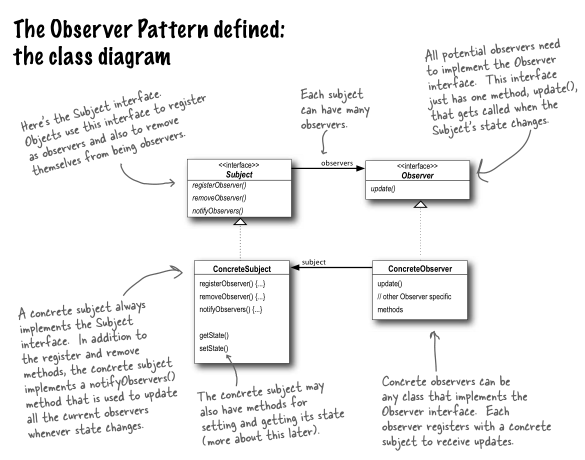
\includegraphics[width=\linewidth]{observer/img/observerUML}
	\caption{UML-Darstellung des Observer-Musters}
	\label{fig:observerUML}
\end{figure}
